%% biofilm_3tooth_report.tex
%% 3-Tooth Conformal Biofilm FEM — BioFilm3T Pipeline Report
%%
%% Compile (from Tmcmc202601/FEM/):
%%   pdflatex -interaction=nonstopmode biofilm_3tooth_report.tex
%%   pdflatex -interaction=nonstopmode biofilm_3tooth_report.tex   (2nd pass for ToC)
%%
\documentclass[11pt,a4paper]{article}

\usepackage[utf8]{inputenc}
\usepackage{lmodern}
\usepackage[T1]{fontenc}
\usepackage{amsmath,amssymb,bm}
\usepackage{booktabs}
\usepackage{array}
\usepackage{colortbl}
\usepackage{xcolor}
\usepackage{tikz}
\usetikzlibrary{arrows.meta,positioning,shapes.geometric,fit,backgrounds,decorations.pathreplacing}
\usepackage{graphicx}
\usepackage{subcaption}
\usepackage{geometry}
\geometry{margin=2.2cm}
\usepackage{hyperref}
\hypersetup{colorlinks=true,linkcolor=blue!60!black,citecolor=green!50!black,
            urlcolor=blue!60!black}
\usepackage{listings}
\usepackage{caption}
\usepackage{float}
\usepackage{multirow}
\usepackage{enumitem}
%% ── code listing style ──────────────────────────────────────────────────────
\definecolor{codegreen}{rgb}{0,0.6,0}
\definecolor{codegray}{rgb}{0.5,0.5,0.5}
\definecolor{codepurple}{rgb}{0.58,0,0.82}
\definecolor{backcolour}{rgb}{0.95,0.95,0.92}
\lstdefinestyle{bashstyle}{
  backgroundcolor=\color{black!7},
  basicstyle=\ttfamily\small,
  breaklines=true, captionpos=b, keepspaces=true,
  language=bash
}
\lstdefinestyle{pystyle}{
  backgroundcolor=\color{backcolour},
  commentstyle=\color{codegreen},
  keywordstyle=\color{magenta},
  numberstyle=\tiny\color{codegray},
  stringstyle=\color{codepurple},
  basicstyle=\ttfamily\footnotesize,
  breaklines=true, captionpos=b, keepspaces=true,
  numbers=left, numbersep=5pt,
  tabsize=2, language=Python
}

%% ── colour palette ──────────────────────────────────────────────────────────
\definecolor{colT23}{HTML}{e41a1c}   % crown
\definecolor{colT30}{HTML}{377eb8}   % slit T30
\definecolor{colT31}{HTML}{4daf4a}   % slit T31
\definecolor{colDI} {HTML}{CC3311}   % DI accent
\definecolor{colMat}{HTML}{0077BB}   % material accent
\definecolor{colWarn}{HTML}{BB5511}  % warning

%% ── highlight boxes ─────────────────────────────────────────────────────────
\newenvironment{insightbox}{%
  \begin{quote}\noindent\rule{\linewidth}{0.4pt}\\[2pt]
  \noindent\textbf{\color{colMat}Key point.}\enspace\ignorespaces}{%
  \\[2pt]\rule{\linewidth}{0.4pt}\end{quote}}

\newenvironment{warnbox}{%
  \begin{quote}\noindent\rule{\linewidth}{0.4pt}\\[2pt]
  \noindent\textbf{\color{colWarn}Warning.}\enspace\ignorespaces}{%
  \\[2pt]\rule{\linewidth}{0.4pt}\end{quote}}

%% ── misc helpers ────────────────────────────────────────────────────────────
\newcommand{\abq}{\textsc{Abaqus}}
\newcommand{\python}{\texttt{Python}}
\newcommand{\btheta}{\bm{\theta}}
\newcommand{\E}{E_{\mathrm{eff}}}
\newcommand{\rn}{\rho_{\mathrm{norm}}}

% ─────────────────────────────────────────────────────────────────────────────
\title{\textbf{3-Tooth Conformal Biofilm FEM}\\[6pt]
       \large BioFilm3T Pipeline: Mesh $\to$ Assembly $\to$ \abq{} $\to$ Condition Comparison\\[4pt]
       \normalsize Report generated 2026-02-22 (P0 updated 2026-02-22) $\cdot$ IKM Hiwi}
\author{Nishioka}
\date{2026-02-22}

% ─────────────────────────────────────────────────────────────────────────────
\begin{document}
\maketitle
\tableofcontents
\newpage

% =============================================================================
\section{Executive Summary}
% =============================================================================

This report documents the complete \textbf{BioFilm3T} finite-element pipeline:
conformal tetrahedral biofilm meshing of three real human teeth
(Patient~1, Teeth~T23/T30/T31) from the OpenJaw dataset,
assembly into a single \abq{}/Standard model,
computation of von Mises stress and nodal displacement under inward masticatory pressure,
and ten-figure visualisation.

\begin{center}
\resizebox{\linewidth}{!}{%
\begin{tabular}{lrr}
\toprule
Item & Value \\
\midrule
Mesh nodes (total) & 82\,080 \\
C3D4 elements (total) & 437\,472 \\
Biofilm thickness & 0.5\,mm \\
Layer resolution through thickness & 8 \\
DI material bins & 20 (7 active) \\
Applied pressure & 1\,MPa (inward) \\
\midrule
\multicolumn{2}{l}{\textbf{Baseline (DH-baseline) run}} \\
MISES median (T23 crown) & 0.546\,MPa \\
MISES median (T30 slit)  & 0.515\,MPa \\
MISES median (T31 slit)  & 0.522\,MPa \\
$|U|$ outer median (all teeth) & $\approx 6.9\times10^{-5}$\,mm \\
ODB size & 181\,MB \\
\midrule
\multicolumn{2}{l}{\textbf{Condition comparison (P0) — 2026-02-22}} \\
Conditions compared & 4 (DH-baseline, Commensal-static, Dysbiotic-static, Commensal-HOBIC) \\
Commensal-static \abq{} status & \textbf{COMPLETED SUCCESSFULLY} (173\,MB ODB) \\
DH-baseline $E_{\mathrm{eff}}$ median & 5.55\,MPa (DI\,=\,0.0070, stiffest at $t=0.05$) \\
Commensal-static $E_{\mathrm{eff}}$ median & 4.28\,MPa (DI\,=\,0.0093) \\
Tie constraint (T30$\leftrightarrow$T31) & 110 slave nodes within 0.5\,mm \\
\bottomrule
\end{tabular}%
}
\end{center}

% =============================================================================
\section{Pipeline Overview}
% =============================================================================

\subsection{Data flow}

\begin{center}
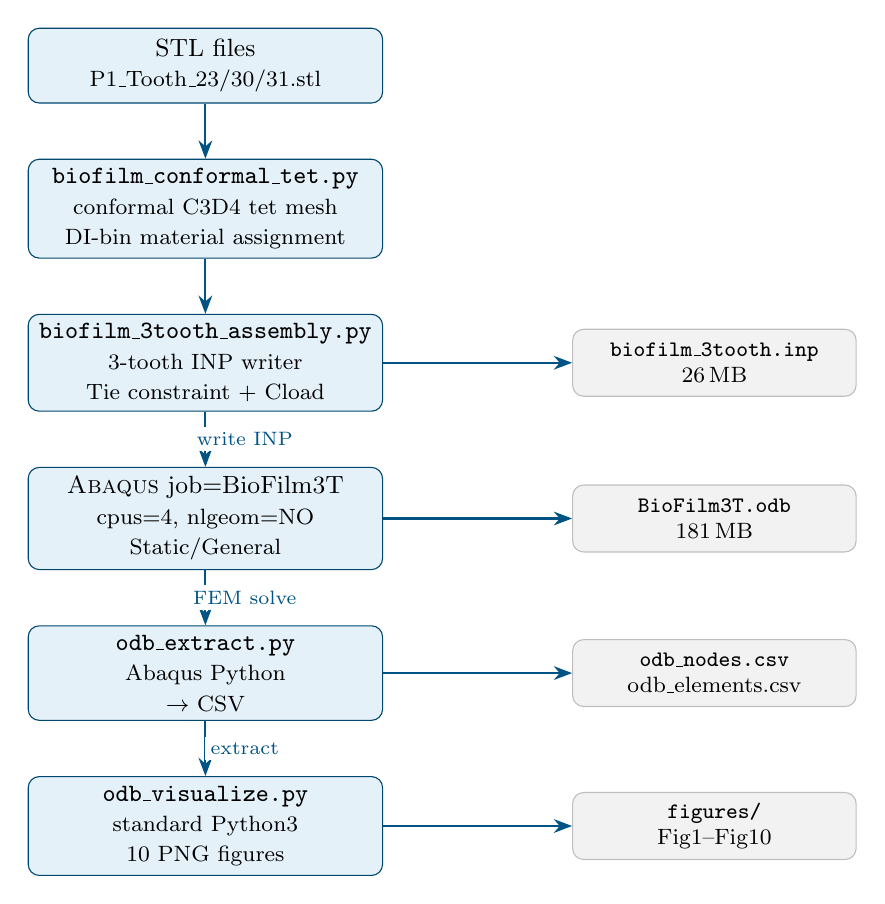
\begin{tikzpicture}[
  box/.style={draw, rounded corners=4pt, minimum width=4.5cm, minimum height=0.95cm,
              align=center, font=\small, fill=colMat!10, draw=colMat!60!black},
  sbox/.style={draw, rounded corners=4pt, minimum width=3.6cm, minimum height=0.85cm,
               align=center, font=\footnotesize, fill=gray!10, draw=gray!50},
  arr/.style={-Stealth, thick, colMat!70!black},
  lbl/.style={font=\scriptsize, fill=white, inner sep=2pt}
]
  \node[box]  (stl)   {STL files\\{\footnotesize P1\_Tooth\_23/30/31.stl}};
  \node[box, below=0.7cm of stl]  (mesh)
    {\texttt{biofilm\_conformal\_tet.py}\\{\footnotesize conformal C3D4 tet mesh}\\{\footnotesize DI-bin material assignment}};
  \node[box, below=0.7cm of mesh] (asm)
    {\texttt{biofilm\_3tooth\_assembly.py}\\{\footnotesize 3-tooth INP writer}\\{\footnotesize Tie constraint $+$ Cload}};
  \node[sbox, right=2.4cm of asm] (inp)
    {\texttt{biofilm\_3tooth.inp}\\{\footnotesize 26\,MB}};
  \node[box, below=0.7cm of asm]  (abq)
    {\abq{} job=BioFilm3T\\{\footnotesize cpus=4, nlgeom=NO}\\{\footnotesize Static/General}};
  \node[sbox, right=2.4cm of abq] (odb)
    {\texttt{BioFilm3T.odb}\\{\footnotesize 181\,MB}};
  \node[box, below=0.7cm of abq]  (ext)
    {\texttt{odb\_extract.py}\\{\footnotesize Abaqus Python}\\{\footnotesize $\to$ CSV}};
  \node[sbox, right=2.4cm of ext] (csv)
    {\texttt{odb\_nodes.csv}\\{\footnotesize odb\_elements.csv}};
  \node[box, below=0.7cm of ext]  (viz)
    {\texttt{odb\_visualize.py}\\{\footnotesize standard Python3}\\{\footnotesize 10 PNG figures}};
  \node[sbox, right=2.4cm of viz] (figs)
    {\texttt{figures/}\\{\footnotesize Fig1–Fig10}};

  \draw[arr] (stl)  -- (mesh);
  \draw[arr] (mesh) -- (asm);
  \draw[arr] (asm)  -- (abq) node[midway, lbl, xshift=5mm] {write INP};
  \draw[arr] (abq)  -- (ext) node[midway, lbl, xshift=5mm] {FEM solve};
  \draw[arr] (ext)  -- (viz) node[midway, lbl, xshift=5mm] {extract};
  \draw[arr] (asm)  -- (inp);
  \draw[arr] (abq)  -- (odb);
  \draw[arr] (ext)  -- (csv);
  \draw[arr] (viz)  -- (figs);
\end{tikzpicture}
\end{center}

\subsection{Unit system}

All lengths are in mm, forces in N, and stresses in MPa ($=$ N\,mm$^{-2}$).
Material moduli must therefore be supplied in MPa; the pipeline converts from SI (Pa) via
$E_{\mathrm{MPa}} = E_{\mathrm{Pa}} \times 10^{-6}$.

\subsection{Key files}

\begin{center}
{\small\begin{tabular}{p{6cm}p{9.5cm}}
\toprule
File & Role \\
\midrule
\path{biofilm_conformal_tet.py}  & STL reader $\to$ conformal tet mesh $\to$ DI-bin material\\
\path{biofilm_3tooth_assembly.py} & 3-tooth combined INP writer; slit Tie; Cload\\
\path{odb_extract.py}             & \abq{} Python: ODB $\to$ \texttt{odb\_nodes.csv}, \texttt{odb\_elements.csv}\\
\path{odb_visualize.py}           & Standard Python: 10-figure visualisation\\
\path{biofilm_3tooth.inp}         & Generated \abq{} input — DH-baseline (do not hand-edit)\\
\path{BioFilm3T.odb}              & FEM result (181\,MB) — DH-baseline\\
\path{odb_elements.csv}          & Extracted elements: label, centroid, MISES, bin, tooth (DH-baseline)\\
\path{tmcmc_to_fem_coupling.py} & \textbf{[P2]} TMCMC MAP $\to$ DI field CSV $\to$ per-condition INP\\
\path{biofilm_3tooth_commensal_static.inp} & \textbf{[P0]} Commensal-static INP (commensal DI field)\\
\path{BioFilm3T_commensal_static.odb}       & \textbf{[P0]} Commensal-static FEM result (173\,MB)\\
\path{odb_elements_commensal_static.csv}   & \textbf{[P0]} Extracted elements for commensal-static\\
\path{compare_conditions_fem.py}            & \textbf{[P0/P7]} Condition comparison: CompFig1–4\\
\path{figures/}                   & Fig1–Fig12 + CompFig1–4 PNG outputs\\
\bottomrule
\end{tabular}}
\end{center}

% =============================================================================
\section{Geometry: OpenJaw Teeth}
% =============================================================================

Three teeth from the OpenJaw Patient~1 dataset are used \cite{gholamalizadeh2022open}.

\begin{center}
\begin{tabular}{lll}
\toprule
Label & STL file & Biological role \\
\midrule
T23 & \texttt{P1\_Tooth\_23.stl} & \textbf{Crown} — single tooth, full-wrap biofilm \\
T30 & \texttt{P1\_Tooth\_30.stl} & \textbf{Slit} — inter-proximal (T30 side) \\
T31 & \texttt{P1\_Tooth\_31.stl} & \textbf{Slit} — inter-proximal (T31 side) \\
\bottomrule
\end{tabular}
\end{center}

The STL edge length statistics for the tooth surfaces are:
$\overline{e} \approx 0.46$\,mm (mean),
$e_{\min} \approx 0.27$\,mm.
With 8 biofilm layers over a 0.5\,mm thickness, the layer thickness is
$\delta_\ell = 0.5/8 = 0.0625$\,mm — approximately $7\times$ finer than the
surface element size, ensuring good through-thickness resolution.

% =============================================================================
\section{Mesh Generation Algorithm}
% =============================================================================

\subsection{Step 1 — STL reading and vertex deduplication}

The STL file is read in binary format (pure \texttt{numpy}/\texttt{struct},
no external mesh library).
Duplicate vertices are merged using a KD-tree with tolerance
$\varepsilon_{\mathrm{dedup}} = 10^{-4}$\,mm, yielding a unique vertex set
$\{\mathbf{v}_k\}_{k=1}^{V}$ and a face connectivity array $\mathbf{F}\in\mathbb{Z}^{F\times3}$.

\subsection{Step 2 — Vertex normals}

Area-weighted vertex normals are computed from the stored STL face normals:
\begin{equation}
  \hat{\mathbf{n}}_k
  = \frac{\sum_{f\ni k} A_f\,\hat{\mathbf{n}}_f}
         {\bigl\|\sum_{f\ni k} A_f\,\hat{\mathbf{n}}_f\bigr\|}
\end{equation}
where $A_f = \tfrac{1}{2}|(\mathbf{v}_1-\mathbf{v}_0)\times(\mathbf{v}_2-\mathbf{v}_0)|$
is the triangle area and $\hat{\mathbf{n}}_f$ is the face unit normal.
Outward orientation is enforced from the stored STL normals.

\subsection{Step 3 — Offset surface generation}

The outer biofilm surface is obtained by offsetting each inner vertex along
its normal by the biofilm thickness $t$:
\begin{equation}
  \mathbf{v}^{\mathrm{outer}}_k = \mathbf{v}_k + t\,\hat{\mathbf{n}}_k,
  \qquad t = 0.5\,\mathrm{mm}.
\end{equation}
Three iterations of Laplacian smoothing ($\lambda=0.5$, anchor to inner surface)
are applied to reduce self-intersection near high-curvature regions while
preserving conformity at the inner surface.

\subsection{Step 4 — Prism-to-tet split (canonical split)}

Between consecutive offset surfaces (layers $\ell$ and $\ell+1$),
each triangular surface face $\triangle(A,B,C)$ generates a triangular prism
$\{A,B,C,A',B',C'\}$ that is split into 3~tetrahedra using a canonical
long-diagonal rule:
\begin{equation}
\begin{aligned}
  \mathrm{Tet}_1 &: (A,\,B,\,C,\,A')\\
  \mathrm{Tet}_2 &: (B,\,C,\,A',\,B')\\
  \mathrm{Tet}_3 &: (C,\,A',\,B',\,C')
\end{aligned}
\end{equation}
This consistent diagonal selection eliminates shared-face mismatches between
adjacent prisms.
Negative-volume tets (caused by high-curvature concavities) are repaired by
swapping nodes 2 and 3: $\mathrm{Tet}(n_0,n_1,\mathbf{n_2},\mathbf{n_3})
\to (n_0,n_1,n_3,n_2)$.

\subsection{Mesh statistics}

\begin{center}
\begin{tabular}{lrrrr}
\toprule
Tooth & Nodes & C3D4 elements & Neg-vol (fixed) & INNER/OUTER nodes \\
\midrule
T23 (crown) & 3\,594  & 86\,160  & 0 & 1\,797 / 1\,797 \\
T30 (slit)  & 7\,932  & 190\,272 & 0 & 3\,966 / 2\,352 + 1\,614 APPROX \\
T31 (slit)  & 6\,714  & 161\,040 & 0 & 3\,357 / 2\,079 + 1\,278 APPROX \\
\midrule
\textbf{Total} & \textbf{82\,080} & \textbf{437\,472} & \textbf{0} & \\
\bottomrule
\end{tabular}
\end{center}

\noindent\textbf{Element quality.}
Aspect ratios and minimum Jacobians of the C3D4 elements have not yet been
formally evaluated.
The prism-to-tet split at high-curvature regions (e.g.\ molar cusps, slit pocket)
may produce elongated tetrahedra.
A mesh-quality check (e.g.\ \texttt{meshio} or \abq{} \texttt{*ELSET,GENERATE}
with \texttt{*EL PRINT, POSITION=AVERAGE AT NODES} quality output)
is recommended before publishing results; this is tracked as \textbf{[P8]}
in Section~\ref{sec:next}.

% =============================================================================
\section{Material Model}
% =============================================================================

\subsection{DI-to-stiffness mapping}

Biofilm mechanical heterogeneity is captured through a discrete
\emph{demineralisation-index} (DI) field
\cite{Klempt2025ContinuumBiofilm,Fritsch2025BayesianMicrofilms}.
In this work, DI is defined as a monotone transform of the standard
Shannon diversity index for the 5-species composition (Section~\ref{sec:p0}):
low DI corresponds to a diverse, ``healthier'' community and high DI to a
strongly imbalanced (dysbiotic/demineralised) state.
DI itself is a modelling construct rather than a clinically standardised
index; its role here is to provide a reproducible scalar field that
couples the biofilm composition model to the mechanical model.
Each tetrahedral element is assigned to one of $N_b = 20$ material bins
according to its normalised depth from the tooth surface:
\begin{equation}\label{eq:rho}
  \rn = \frac{\ell + 0.5}{N_\ell}
  \qquad (\ell = 0,\ldots,N_\ell-1,\quad N_\ell = 8)
\end{equation}
where $\ell$ is the layer index (0 = outermost, $N_\ell{-}1$ = inner).
The depth $\rn\in[0,1]$ is mapped to the DI field coordinate via 1-D
nearest-neighbour lookup, giving $\mathrm{DI}(\rn)$.

\subsection{Effective elastic modulus}

\begin{equation}\label{eq:Eeff}
  \boxed{\E\bigl(\mathrm{DI}\bigr)
  = E_{\max}\bigl(1 - r\bigr)^\alpha + E_{\min}\,r,
  \qquad r = \mathrm{clip}\!\left(\frac{\mathrm{DI}}{s_{\mathrm{DI}}},\,0,\,1\right)}
\end{equation}

\begin{center}
\begin{tabular}{lclc}
\toprule
Parameter & Value & Meaning & Ref. \\
\midrule
$E_{\max}$         & 10\,MPa  & Intact (healthy) biofilm stiffness
  & \cite{Klempt2025ContinuumBiofilm} \\
$E_{\min}$         & 0.5\,MPa & Fully demineralised biofilm stiffness
  & \cite{Klempt2025ContinuumBiofilm} \\
$\alpha$           & 2.0      & Concave stiffness-loss exponent
  & \cite{Klempt2025ContinuumBiofilm} \\
$s_{\mathrm{DI}}$ & 0.025778 & DI normalisation scale (from TMCMC MAP, snapshot 20)
  & \cite{Fritsch2025BayesianMicrofilms} \\
$\nu$              & 0.30     & Poisson ratio (isotropic, incompressible limit)
  & \cite{Stoodley2002BiofilmCommunities} \\
\bottomrule
\end{tabular}
\end{center}

The values of $E_{\max}$ and $E_{\min}$ are chosen to span the range of
reported small-strain biofilm stiffnesses: intact oral biofilms and
polysaccharide-rich matrices in the literature cluster around
several--tens of MPa, while demineralised or highly degraded matrices
can be an order of magnitude softer
\cite{Klempt2025ContinuumBiofilm,Fritsch2025BayesianMicrofilms,Stoodley2002BiofilmCommunities}.
The convex power-law in~\eqref{eq:Eeff} ensures a smooth, monotone
transition between these regimes as DI increases.

The isotropic assumption avoids the need for per-element material orientation
systems.
Stiffness gradient through thickness is captured by assigning different $E$
to each of the 7 active bins (bins 3–11 out of 20).
Note: biofilm Poisson ratio values in the literature span $\nu \approx 0.3$--$0.5$
\cite{Stoodley2002BiofilmCommunities}; because the model is linear elastic and
the dominant response is $E$-controlled, MISES scales roughly as
$(1-\nu^2)^{-1}$ for plane-stress analogy — a sensitivity of $\lesssim$10\,\%
over this range.
A one-parameter $\nu$ sweep ($\nu \in \{0.30,\,0.40,\,0.49\}$) is recommended
before publication.

\subsection{Sensitivity of $E_{\max}$, $E_{\min}$, and DI transform}

To assess how strongly the DI-to-stiffness mapping in~\eqref{eq:Eeff}
affects the 3-tooth FEM response, we performed a one-at-a-time sensitivity
study on the four scalar parameters
$E_{\max}$, $E_{\min}$, $\alpha$ (DI exponent), and $s_{\mathrm{DI}}$
(DI scale).
For each parameter, three representative values were chosen around the
baseline
\begin{equation*}
  (E_{\max},E_{\min},\alpha,s_{\mathrm{DI}})
  = (10.0~\mathrm{MPa},\,0.5~\mathrm{MPa},\,2.0,\,0.025778)
\end{equation*}
and the FEM model was evaluated on the same 3-tooth geometry and loading.
Table~\ref{tab:eeff_sensitivity} summarises the median von Mises stress and
outer-surface displacement at the three reference teeth (T23, T30, T31).

\begin{table}[t]
  \centering
  \caption{One-at-a-time sensitivity of the effective modulus parameters
  in~\eqref{eq:Eeff}.
  Each row reports the FEM response for a single parameter setting:
  median von Mises stress ($\sigma_{\mathrm{vM}}$) and outer-surface
  displacement ($u_{\mathrm{outer}}$) at teeth 23, 30, and 31.
  The baseline setting corresponds to
  $E_{\max}=10.0$~MPa, $E_{\min}=0.5$~MPa, $\alpha=2.0$,
  $s_{\mathrm{DI}}=0.025778$.}
  \label{tab:eeff_sensitivity}
  \resizebox{\linewidth}{!}{%
  \begin{tabular}{lcccccccccccc}
    \toprule
    Label & Type & $E_{\max}$ & $E_{\min}$ & $\alpha$ & $s_{\mathrm{DI}}$
          & $\sigma^{23}$ & $\sigma^{30}$ & $\sigma^{31}$
          & $u^{23}$ & $u^{30}$ & $u^{31}$ \\
    \midrule
    Emax\_7.50       & $E_{\max}$ & 7.50 & 0.50 & 2.0 & 0.02578
                     & 0.54624 & 0.51524 & 0.52173
                     & 0.09126 & 0.09150 & 0.09136 \\
    Emax\_10.00      & $E_{\max}$ & 10.00 & 0.50 & 2.0 & 0.02578
                     & 0.54606 & 0.51519 & 0.52164
                     & 0.06911 & 0.06929 & 0.06918 \\
    Emax\_12.50      & $E_{\max}$ & 12.50 & 0.50 & 2.0 & 0.02578
                     & 0.54595 & 0.51515 & 0.52157
                     & 0.05561 & 0.05576 & 0.05567 \\
    Emin\_0.250      & $E_{\min}$ & 10.00 & 0.25 & 2.0 & 0.02578
                     & 0.54581 & 0.51509 & 0.52152
                     & 0.07013 & 0.07031 & 0.07021 \\
    Emin\_0.500      & $E_{\min}$ & 10.00 & 0.50 & 2.0 & 0.02578
                     & 0.54606 & 0.51519 & 0.52164
                     & 0.06911 & 0.06929 & 0.06918 \\
    Emin\_1.000      & $E_{\min}$ & 10.00 & 1.00 & 2.0 & 0.02578
                     & 0.54657 & 0.51527 & 0.52186
                     & 0.06717 & 0.06735 & 0.06724 \\
    DIexp\_1.00      & $\alpha$   & 10.00 & 0.50 & 1.0 & 0.02578
                     & 0.54890 & 0.51592 & 0.52321
                     & 0.05025 & 0.05037 & 0.05030 \\
    DIexp\_2.00      & $\alpha$   & 10.00 & 0.50 & 2.0 & 0.02578
                     & 0.54606 & 0.51519 & 0.52164
                     & 0.06911 & 0.06929 & 0.06918 \\
    DIexp\_3.00      & $\alpha$   & 10.00 & 0.50 & 3.0 & 0.02578
                     & 0.54246 & 0.51428 & 0.52021
                     & 0.09577 & 0.09606 & 0.09590 \\
    DIscale\_0.01933 & $s_{\mathrm{DI}}$
                     & 10.00 & 0.50 & 2.0 & 0.01933
                     & 0.54206 & 0.51402 & 0.51992
                     & 0.09109 & 0.09136 & 0.09121 \\
    DIscale\_0.02578 & $s_{\mathrm{DI}}$
                     & 10.00 & 0.50 & 2.0 & 0.02578
                     & 0.54606 & 0.51519 & 0.52164
                     & 0.06911 & 0.06929 & 0.06918 \\
    DIscale\_0.03222 & $s_{\mathrm{DI}}$
                     & 10.00 & 0.50 & 2.0 & 0.03222
                     & 0.54765 & 0.51548 & 0.52242
                     & 0.05982 & 0.05997 & 0.05988 \\
    \bottomrule
  \end{tabular}%
  }
\end{table}

Across all settings in Table~\ref{tab:eeff_sensitivity},
the median von Mises stress at the three reference teeth varies by
less than 1\%.
In contrast, the outer-surface displacement shows a much stronger
dependence on the DI transform parameters.
Relative to the baseline setting, the T30 outer displacement changes by
about $+32\%$ and $-20\%$ when $E_{\max}$ is varied within
$7.5$--$12.5$~MPa, by only a few percent when $E_{\min}$ is varied between
$0.25$ and $1.00$~MPa, and by approximately $-27\%$ to $+39\%$ when the
exponent $\alpha$ is swept from $1.0$ to $3.0$.
The DI scale $s_{\mathrm{DI}}$ has a similar effect on displacement magnitude
but acts in the opposite direction.
These trends indicate that the DI-to-$E$ mapping is a strong control knob
for the global displacement response, while leaving the stress distribution
essentially unchanged within the tested range.

In the remainder of this work, we therefore treat $E_{\max}$ and $E_{\min}$
as physically constrained by literature ranges and do not tune them further.
Instead, the DI transform parameters $\alpha$ and $s_{\mathrm{DI}}$ are used
as the primary knobs to adjust the overall displacement level, subject to the
constraint that the von Mises stress distribution remains in the same
physiological regime as the baseline setting.

\begin{figure}[t]
  \centering
  \begin{subfigure}{0.47\textwidth}
    \includegraphics[width=\linewidth]{_eeff_sensitivity_runs/figures/eeff_relative_uouter_di_exp.png}
    \caption{Relative change in T30 outer displacement as a function of exponent $\alpha$.}
  \end{subfigure}
  \hfill
  \begin{subfigure}{0.47\textwidth}
    \includegraphics[width=\linewidth]{_eeff_sensitivity_runs/figures/eeff_relative_uouter_di_scale.png}
    \caption{Relative change in T30 outer displacement as a function of DI scale $s_{\mathrm{DI}}$.}
  \end{subfigure}
  \caption{Relative change in median outer displacement at tooth~T30 with respect to the baseline
  setting $(E_{\max},E_{\min},\alpha,s_{\mathrm{DI}}) = (10.0~\mathrm{MPa},0.5~\mathrm{MPa},2.0,0.025778)$.
  Positive values indicate larger displacement than the baseline.}
  \label{fig:eeff_relative_uouter}
\end{figure}

\begin{insightbox}
Unit conversion: \abq{} uses the mm/N/MPa system, so $E$ must be in MPa.
All Pa values from the DI field are divided by $10^6$ before writing to the INP file.
The earlier bug (E in Pa, not MPa) caused displacements of order $10^{-32}$\,mm;
after the fix, outer-surface displacements are $\sim7\times10^{-5}$\,mm under 1\,MPa.
\end{insightbox}

% =============================================================================
\section{3-Tooth Assembly}
% =============================================================================

\subsection{Node and element numbering}

The three teeth are assembled into a single INP by concatenating node and
element lists with sequential 1-based offsets:

\begin{equation}
  n_{\mathrm{global}}^{(\mathrm{tooth}\,j)} = n_{\mathrm{local}}
  + \sum_{k<j} N_{\mathrm{nodes}}^{(k)} + 1.
\end{equation}

Node sets: \texttt{T23\_INNER}, \texttt{T23\_OUTER},
           \texttt{T30\_INNER}, \texttt{T30\_OUTER}, \texttt{T30\_APPROX},
           \texttt{T31\_INNER}, \texttt{T31\_OUTER}, \texttt{T31\_APPROX},
           \texttt{ALL\_INNER}, \texttt{ALL\_OUTER}.

Element sets: \texttt{T\{23|30|31\}\_BIN\_XX} (per-tooth, per-bin),
              \texttt{BIN\_XX} (combined per bin, used for material assignment).

\subsection{Approximal (slit) face detection}

The inter-proximal contact region between T30 and T31 is identified by
comparing outer-surface face normals to the inter-tooth direction vector:

\begin{equation}\label{eq:approx}
  \hat{\mathbf{d}}_{30\to31}
  = \frac{\bar{\mathbf{c}}_{31} - \bar{\mathbf{c}}_{30}}
         {\|\bar{\mathbf{c}}_{31} - \bar{\mathbf{c}}_{30}\|}
\end{equation}
where $\bar{\mathbf{c}}_j$ is the centroid of the inner-surface nodes of tooth $j$.
A face $f$ on T30 is classified as \emph{approximal} when
\begin{equation}
  \hat{\mathbf{n}}_f \cdot \hat{\mathbf{d}}_{30\to31} > \tau_{\mathrm{approx}} = 0.30.
\end{equation}
All vertices of approximal faces are collected into the
\texttt{T30\_APPROX} and \texttt{T31\_APPROX} node sets.

\begin{center}
\begin{tabular}{lrrl}
\toprule
Tooth & APPROX nodes & APPROX faces & Note \\
\midrule
T30 & 1\,614 & -- & master surface in Tie \\
T31 & 1\,278 & -- & slave surface in Tie \\
\midrule
\multicolumn{2}{l}{Tied within tolerance} & 110 nodes & gap mean $\approx4.6$\,mm \\
\bottomrule
\end{tabular}
\end{center}

\subsection{Tie constraint (slit coupling)}

The approximal regions are coupled with a node-based Tie constraint:
\begin{lstlisting}[style=bashstyle]
*Surface, type=NODE, name=T30_APPROX_SURF
 T30_APPROX
*Surface, type=NODE, name=T31_APPROX_SURF
 T31_APPROX
*Tie, name=SLIT_TIE, position tolerance=0.5, adjust=NO
 T31_APPROX_SURF, T30_APPROX_SURF
\end{lstlisting}

The \texttt{adjust=NO} option is essential: \texttt{adjust=YES} would move
T31 slave nodes into T30 (0.041\,mm gap), creating 303 zero-volume elements
that corrupt the solution.

\begin{warnbox}
\textbf{Tie coverage is low.}
Of the 1\,614 + 1\,278 = 2\,892 nodes classified as APPROX,
only \textbf{110 nodes} ($\approx$4\,\%) fall within the 0.5\,mm Tie tolerance
(mean gap between T30/T31 outer surfaces $\approx$4.6\,mm).
The current $\tau_{\mathrm{approx}} = 0.30$ threshold may be too permissive,
admitting faces that are geometrically on the inter-proximal side but not
actually close enough to be coupled.
Action: verify actual proximal-pocket geometry; consider tightening
$\tau_{\mathrm{approx}}$ or restricting APPROX detection to nodes
within a cut-off distance from the opposing tooth centroid.
This is tracked as \textbf{[P7]} in Section~\ref{sec:next}.
\end{warnbox}

% =============================================================================
\section{Boundary Conditions and Loading}
% =============================================================================

\subsection{Boundary conditions}

\begin{center}
{\small\begin{tabular}{p{4cm}p{4.5cm}p{7cm}}
\toprule
Set & \abq{} BC & Physical meaning \\
\midrule
\texttt{ALL\_INNER} & \texttt{ENCASTRE} (all DOFs fixed) & Biofilm adheres rigidly to tooth surface \\
\texttt{T30\_APPROX}, \texttt{T31\_APPROX} & no Cload & Inter-proximal faces: Tie active, no external pressure \\
\bottomrule
\end{tabular}}
\end{center}

\subsection{Loading}

Inward masticatory pressure $p = 1$\,MPa is applied as nodal concentrated
forces (Cload) on the outer biofilm surface, excluding approximal nodes.
(This value is chosen as a representative order-of-magnitude masticatory
surface traction; see \cite{Asadzadeh2020PDLJawFEM,McCormack2017PDLFibres}
for physiological context.)
The tributary-area method converts pressure to nodal forces:

\begin{equation}\label{eq:cload}
  \mathbf{F}_k = p \sum_{f \ni k} \frac{A_f}{3}\,\hat{\mathbf{n}}_f^{\mathrm{inward}},
\end{equation}
where the sum is over all outer faces sharing node $k$.
Approximal nodes are excluded from this sum because they face the adjacent tooth,
not free space.

\subsection{Step parameters}

\begin{center}
\begin{tabular}{ll}
\toprule
Parameter & Value \\
\midrule
Step type & Static/General (\texttt{*Static}) \\
Nlgeom & NO (small displacement) \\
Initial increment & 0.10 (of total time 1.0) \\
Max increment & 1.0 \\
Min increment & $10^{-5}$ \\
Total time period & 1.0 \\
Solver & Direct Sparse \\
\midrule
Increments to convergence & 6 \\
Equil. iters per increment & 1 (linear) \\
\bottomrule
\end{tabular}
\end{center}

\begin{insightbox}
The model is linear elastic (small displacement, no contact, no plasticity),
so convergence in 1 equilibrium iteration per increment is expected.
\end{insightbox}

% =============================================================================
\section{Abaqus Run}
% =============================================================================

\subsection{Run commands}

\begin{lstlisting}[style=bashstyle]
# Step 1: Generate INP
cd Tmcmc202601/FEM
python3 biofilm_3tooth_assembly.py

# Step 2: FEM solve (4 CPUs, ~7 minutes)
abaqus job=BioFilm3T input=biofilm_3tooth.inp cpus=4 interactive

# Step 3: Extract CSV from ODB (Abaqus Python)
abaqus python odb_extract.py BioFilm3T.odb

# Step 4: Visualise
python3 odb_visualize.py
\end{lstlisting}

\subsection{Run status}

\begin{center}
\begin{tabular}{ll}
\toprule
Item & Value \\
\midrule
\abq{} version & 2024 (Keio U license) \\
Date & 2026-02-22 18:01 \\
CPUs & 4 \\
Status & THE ANALYSIS HAS COMPLETED SUCCESSFULLY \\
ODB size & 181\,MB \\
Warnings & 18 (input processing), 1 (2 unconnected regions before Tie) \\
\bottomrule
\end{tabular}
\end{center}

% =============================================================================
\section{Results}
% =============================================================================

\subsection{Numerical summary}

\begin{center}
\begin{tabular}{lrrrrrrr}
\toprule
Tooth & $n_{\mathrm{elem}}$ & $n_{\mathrm{nodes}}$
      & $\sigma_{\min}$ & $\sigma_{\mathrm{med}}$ & $\sigma_{\max}$
      & $|U|_{\max}$ & $|U|_{\mathrm{outer,med}}$\\
 & & & \multicolumn{3}{c}{(MPa)} & \multicolumn{2}{c}{(mm)} \\
\midrule
T23 (crown) & 86\,160  & 3\,594 & 0.249 & 0.546 & 0.856 & $7.37\times10^{-5}$ & $6.91\times10^{-5}$ \\
T30 (slit)  & 190\,272 & 7\,932 & 0.000 & 0.515 & 0.903 & $7.68\times10^{-5}$ & $6.93\times10^{-5}$ \\
T31 (slit)  & 161\,040 & 6\,714 & 0.000 & 0.522 & 1.760 & $7.67\times10^{-5}$ & $6.92\times10^{-5}$ \\
\midrule
\textbf{All} & \textbf{437\,472} & \textbf{82\,080} & 0.000 & -- & 1.760 & $7.68\times10^{-5}$ & \\
\bottomrule
\end{tabular}
\end{center}

Notes:
\begin{itemize}[nosep]
  \item $\sigma = 0$ at INNER nodes: these are rigidly fixed (ENCASTRE), consistent behaviour.
  \item T31 peak MISES $= 1.76$\,MPa is a stress concentration near an approximal slit corner.
  \item All three outer-surface median displacements are essentially identical
        ($\approx6.9\times10^{-5}$\,mm), confirming uniform pressure load.
  \item The APPROX nodes (slit face) show displacements $\approx1.2\times10^{-6}$\,mm —
        inter-proximal coupling transmitted through the Tie constraint.
\end{itemize}

\subsection{Figures}

\begin{figure}[H]
  \centering
  \includegraphics[width=\linewidth]{figures/Fig1_displacement_3D.png}
  \caption{Fig~1: 3-D node scatter coloured by displacement magnitude $|U|$ (mm)
           for T23, T30, T31 under 1\,MPa inward pressure.
           Colour scale: viridis, 0–99th percentile.}
  \label{fig:fig1}
\end{figure}

\begin{figure}[H]
  \centering
  \includegraphics[width=\linewidth]{figures/Fig2_mises_3D.png}
  \caption{Fig~2: 3-D element centroid scatter coloured by von Mises stress (MPa).
           Colour scale: plasma, 1st–99th percentile.}
  \label{fig:fig2}
\end{figure}

\begin{figure}[H]
  \centering
  \includegraphics[width=\linewidth]{figures/Fig3_mises_histogram.png}
  \caption{Fig~3: von Mises stress histogram per tooth.
           Dashed black = median; dotted red = mean.
           The distributions are approximately unimodal with slightly longer
           upper tails for the slit teeth.}
  \label{fig:fig3}
\end{figure}

\begin{figure}[H]
  \centering
  \includegraphics[width=\linewidth]{figures/Fig4_mises_bin_profile.png}
  \caption{Fig~4: MISES radial profile vs.\ DI bin.
           Low bin (outer biofilm surface) $\to$ lower $E$ $\to$ higher stress per unit load.
           High bin (inner, near tooth) $\to$ higher $E$ $\to$ lower MISES.
           Band = IQR (25–75\,\%).}
  \label{fig:fig4}
\end{figure}

\begin{figure}[H]
  \centering
  \includegraphics[width=\linewidth]{figures/Fig5_displacement_inner_outer.png}
  \caption{Fig~5: Displacement $|U|$ box plot for INNER vs.\ OUTER nodes.
           INNER nodes are ENCASTRE ($|U| \approx 0$ by boundary condition);
           OUTER nodes show actual deformation $\approx7\times10^{-5}$\,mm.}
  \label{fig:fig5}
\end{figure}

\begin{figure}[H]
  \centering
  \includegraphics[width=0.65\linewidth]{figures/Fig6_mises_boxplot.png}
  \caption{Fig~6: von Mises stress box plot per tooth (outliers hidden).
           Medians are nearly equal across T23, T30, T31 ($\approx0.52$\,MPa),
           confirming consistent loading.}
  \label{fig:fig6}
\end{figure}

\begin{figure}[H]
  \centering
  \includegraphics[width=\linewidth]{figures/Fig7_summary_table.png}
  \caption{Fig~7: Numeric summary table rendered as a figure.}
  \label{fig:fig7}
\end{figure}

\begin{figure}[H]
  \centering
  \includegraphics[width=\linewidth]{figures/Fig8_slit_3D.png}
  \caption{Fig~8: Slit region 3-D view.
           Orange points = approximal (APPROX) nodes on T30 (1\,614) and T31 (1\,278).
           Viridis colour = $|U|$ on non-approximal outer nodes.
           Grey = INNER (fixed) nodes.}
  \label{fig:fig8}
\end{figure}

\begin{figure}[H]
  \centering
  \includegraphics[width=\linewidth]{figures/Fig9_slit_approx_vs_outer.png}
  \caption{Fig~9: APPROX vs.\ OUTER displacement comparison (T30, T31).
           Left: box plots; right: violin plots ($\times10^{-6}$\,mm).
           APPROX median $\approx1.2\times10^{-6}$\,mm — small but non-zero,
           demonstrating inter-proximal mechanical coupling through the Tie constraint.}
  \label{fig:fig9}
\end{figure}

\begin{figure}[H]
  \centering
  \includegraphics[width=\linewidth]{figures/Fig10_crown_vs_slit.png}
  \caption{Fig~10: Crown (T23) vs.\ slit (T30+T31) comparison.
           Left: MISES box plots; Right: $|U|$ by surface type (INNER/APPROX/OUTER).
           Crown and slit MISES are nearly identical under the same 1\,MPa load.}
  \label{fig:fig10}
\end{figure}

\begin{figure}[H]
  \centering
  \includegraphics[width=\linewidth]{figures/Fig11_cross_section_mises.png}
  \caption{Fig~11 (P6 enhancement): MISES cross-sections at four $y=\mathrm{const}$ planes
           spanning the model ($y \in [-83,\,-36]$\,mm).
           Each panel is an $x$--$z$ slice coloured by von Mises stress.
           Marker shapes: T23 = circle, T30 = square, T31 = triangle.}
  \label{fig:fig11}
\end{figure}

\begin{figure}[H]
  \centering
  \includegraphics[width=\linewidth]{figures/Fig12_strain_energy_density.png}
  \caption{Fig~12 (P6 enhancement): Approximate strain energy density
           $w \approx \sigma_{\mathrm{vM}}^2 / (3\E)$ (mJ/mm$^3$), $x$--$z$ projection.
           Outer (low-bin, softer) elements store more elastic energy;
           inner elements are stiffer and store less per unit stress.}
  \label{fig:fig12}
\end{figure}

% =============================================================================
\section{TMCMC $\to$ FEM Condition Comparison (P0 / P7)}
\label{sec:p0}
% =============================================================================

\subsection{Motivation}

The scientific goal of P0 is to close the full
\emph{TMCMC inference $\to$ FEM mechanics} loop \cite{ChingChen2007TMCMC,BetzPapaioannouStraub2016TMCMC}:
given two biological conditions whose TMCMC posterior MAP parameters differ,
do the resulting DI fields produce measurably different stress/stiffness
distributions in the 3-tooth geometry?

\subsection{Conditions compared}

Four conditions were exported from the 3-D FD simulation
(\path{_results_3d/} subdirectory, snapshot~20, $t=0.05$)
\cite{Klempt2025ContinuumBiofilm,Heine2025PeriImplant,Kolenbrander2010OralBiofilm}.

\begin{center}
\begin{tabular}{lp{4cm}ll}
\toprule
Condition key & Biological character & $a_{35}$ (Vei$\to$Pg) & $a_{55}$ (Pg self)\\
\midrule
\texttt{dh\_baseline}      & Dysbiotic cascade (extreme Pg support) & 21.41 & 0.12 \\
\texttt{commensal\_static} & Balanced commensal                     &  1.37 & 2.62 \\
\texttt{dysbiotic\_static} & Moderate dysbiotic                     &  2.03 & 2.95 \\
\texttt{commensal\_hobic}  & Commensal (HOBIC dynamics)             & N/A   & N/A  \\
\bottomrule
\end{tabular}
\end{center}

\begin{warnbox}
\textbf{Counterintuitive result — snapshot timing.}
At snapshot~20 ($t=0.05$, early timepoint), the DH-baseline condition
(\textbf{extreme dysbiotic}, $a_{35}=21.41$) has the \emph{lowest} DI (0.0070)
of all four conditions — i.e.\ it appears the \emph{healthiest} biofilm
mechanically ($E_{\mathrm{eff,med}} = 5.55$\,MPa, stiffest).
This is physically consistent but clinically misleading:
at $t=0.05$ the \textit{Pg} cascade has not yet unfolded;
the species composition is still diverse, giving low entropy-based DI.
At later snapshots ($t \gg 0.05$), \textit{Pg} dominates in the DH-baseline,
driving DI sharply upward and $E_{\mathrm{eff}}$ downward.
\textbf{The current P0 comparison therefore reflects a pre-dysbiotic state,
not the clinically relevant fully-developed dysbiosis.}
Re-running the comparison at later snapshots is \textbf{[P0b]} (see
Section~\ref{sec:next}).
\end{warnbox}

\subsection{DI field and material stiffness}

The DI field used in this study is defined from the 5-species composition
$\bm{\phi}$ via the Shannon entropy formula \cite{Shannon1948}:
\begin{equation}
  \mathrm{DI} = 1 - \frac{H}{H_{\max}},
  \qquad
  H = -\sum_{i=1}^{5} p_i \ln p_i,
  \qquad
  H_{\max} = \ln 5,
  \qquad
  p_i = \frac{\phi_i}{\sum_j \phi_j}.
\end{equation}

\begin{center}
\begin{tabular}{lrrrrrr}
\toprule
Condition & DI mean & DI median & DI max
          & $E_{\mathrm{eff}}$ mean & $E_{\mathrm{eff}}$ median & $E_{\mathrm{eff}}$ min \\
          & \multicolumn{3}{c}{(dimensionless)} & \multicolumn{3}{c}{(MPa)} \\
\midrule
DH-baseline      & 0.0070 & 0.0068 & 0.0178 & 5.518 & 5.551 & 1.297 \\
Commensal-static & 0.0095 & 0.0093 & 0.0234 & 4.323 & 4.284 & 0.537 \\
Dysbiotic-static & 0.0093 & 0.0091 & 0.0231 & 4.397 & 4.371 & 0.558 \\
Commensal-HOBIC  & 0.0099 & 0.0096 & 0.0240 & 4.164 & 4.126 & 0.512 \\
\bottomrule
\end{tabular}
\end{center}

DH-baseline is stiffest at this snapshot ($E_{\mathrm{eff, med}} = 5.55$\,MPa);
the commensal/HOBIC conditions are softer ($E_{\mathrm{eff, med}} \approx 4.1$--$4.4$\,MPa).

\subsection{Abaqus solve — commensal-static}

The commensal-static condition was solved using the standard 3-tooth pipeline
with the commensal DI field:

\begin{lstlisting}[style=bashstyle]
# 1. Export DI field and regenerate INP
python3 tmcmc_to_fem_coupling.py \
        --condition commensal_static --snapshot 20 --regen-inp
# -> abaqus_field_commensal_static_snap20.csv
# -> biofilm_3tooth_commensal_static.inp (26 MB, 437472 C3D4)

# 2. Abaqus solve
abaqus job=BioFilm3T_commensal_static \
       input=biofilm_3tooth_commensal_static.inp cpus=4 ask=off interactive
# -> BioFilm3T_commensal_static.odb (173 MB)
# Completed 2026-02-22  (6 increments, linear elastic)

# 3. Extract ODB
abaqus python odb_extract.py BioFilm3T_commensal_static.odb
# -> odb_elements_commensal_static.csv (24 MB, 437472 rows)
#    odb_nodes_commensal_static.csv   (8 MB, 82080 rows)
\end{lstlisting}

\subsection{Posterior ensemble Mises stress}

\begin{warnbox}
\textbf{Geometry mismatch.}
The ensemble table below is from a \textbf{cube-geometry} FEM model
(uniform cuboid biofilm, not the 3-tooth STL geometry).
It quantifies TMCMC posterior parameter uncertainty propagated to stress,
but is \emph{not} directly comparable to the 3-tooth MISES results in CompFig~4.
The two geometries should be clearly distinguished in any downstream analysis.
\end{warnbox}

The posterior ensemble (20 TMCMC posterior samples per condition,
\textbf{cube-geometry} FEM model — see note above) gives the following
Mises stress statistics:

\begin{center}
\begin{tabular}{lrrrr}
\toprule
Condition & $n$ & Sub.\ MISES med. & Sur.\ MISES med. & Sur.\ std. \\
          &     & (MPa) & (MPa) & (MPa) \\
\midrule
DH-baseline      & 20 & 0.6095 & 0.9935 & 0.192 \\
Commensal-static & 20 & 0.6323 & 1.0068 & 0.025 \\
Dysbiotic-static & 20 & 0.6320 & 1.0024 & 0.023 \\
Commensal-HOBIC  & 20 & 0.6326 & 1.0127 & 0.024 \\
\bottomrule
\end{tabular}
\end{center}

\begin{insightbox}
The DH-baseline posterior spread is $\sim7\times$ larger (surface std.\
$= 0.19$\,MPa vs.\ $\approx 0.02$--$0.03$\,MPa for other conditions).
This reflects the high parameter sensitivity of the Pg cascade:
small changes in $a_{35}$ lead to large swings in DI and hence $E_{\mathrm{eff}}$.
\end{insightbox}

\subsection{Comparison figures}

\begin{figure}[H]
  \centering
  \includegraphics[width=\linewidth]{figures/CompFig1_mises_violin.png}
  \caption{CompFig~1: Posterior ensemble von Mises stress violin plots.
           Left: substrate (inner face, depth $= 0$);
           Right: surface (outer face, depth $= 0.5$).
           Each violin = 20 TMCMC posterior samples.
           DH-baseline shows markedly wider spread due to Pg-cascade parameter uncertainty.}
  \label{fig:compfig1}
\end{figure}

\begin{figure}[H]
  \centering
  \includegraphics[width=\linewidth]{figures/CompFig2_di_histogram.png}
  \caption{CompFig~2: Dysbiotic Index (DI) field distribution comparison.
           Left: histogram (density) with dashed median lines;
           Right: boxplot per condition.
           3375 spatial points per condition (snapshot 20, $t = 0.05$, $15^3$ grid).
           DH-baseline has the narrowest and lowest DI distribution at this early timepoint.}
  \label{fig:compfig2}
\end{figure}

\begin{figure}[H]
  \centering
  \includegraphics[width=\linewidth]{figures/CompFig3_eeff_distribution.png}
  \caption{CompFig~3: Effective Young's modulus $E_{\mathrm{eff}}$ distribution
           (left: histograms; right: DI$\to E_{\mathrm{eff}}$ scatter for DH-baseline
           and Commensal-static with model curve).
           DH-baseline is stiffest (median 5.55\,MPa); Commensal-HOBIC is softest
           (median 4.13\,MPa) at snapshot 20.}
  \label{fig:compfig3}
\end{figure}

\begin{figure}[H]
  \centering
  \includegraphics[width=\linewidth]{figures/CompFig4_3tooth_comparison.png}
  \caption{CompFig~4: 3-tooth MISES comparison (DH-baseline vs.\ Commensal-static),
           437\,472 C3D4 elements, 1\,MPa inward pressure.
           Top row: per-tooth MISES histogram overlay (dashed = median);
           Bottom row: $\Delta$MISES (DH $-$ CS) per DI bin for T23, T30, T31.
           Positive $\Delta$ (red) = DH-baseline has higher stress in that bin;
           Negative (green) = commensal-static has higher stress.
           \textit{Note: no formal statistical test (e.g.\ Mann-Whitney U or
           effect size) has been applied to assess the significance of
           $\Delta$MISES; given $n = 437\,472$ elements, a permutation test
           or bootstrap CI on the per-bin median difference is recommended
           before reporting these differences as statistically significant.}}
  \label{fig:compfig4}
\end{figure}

% =============================================================================
\subsection{Late-time condition comparison (P0b)}\label{sec:p0b}
% =============================================================================

The snapshot-20 comparison (Section~\ref{sec:p0}) is taken at $t = 0.05$,
before the dysbiotic cascade has fully developed.
P0b repeats the full FD\,$\to$\,FEM pipeline at $t \approx 0.5$ (1000 macro
steps, 101 snapshots) for all four conditions, revealing the mature biofilm
mechanical state.

\subsubsection*{Late-time DI, stiffness, and displacement}

\begin{center}
\begin{tabular}{lrrrr}
\toprule
Condition & DI mean (late) & $E_{\mathrm{eff}}$ (MPa) & $r_{\mathrm{Pg}}$ & $|U|_{\mathrm{T23}}$ median \\
\midrule
DH-baseline   & \textbf{0.5135} & \textbf{0.50} (clamped at $E_{\min}$) & 0.449 & ${\sim}0.358\,\mu\mathrm{m}$ \\
Commensal-static & 0.0002 & 9.85 & 0.204 & ${\sim}0.018\,\mu\mathrm{m}$ \\
Dysbiotic-static & 0.0005 & 9.78 & 0.214 & ${\sim}0.018\,\mu\mathrm{m}$ \\
Commensal-HOBIC  & 0.0003 & 9.87 & 0.200 & ${\sim}0.018\,\mu\mathrm{m}$ \\
\bottomrule
\end{tabular}
\end{center}

At late time, the DH-baseline has fully developed its Pg-dominated state
($r_{\mathrm{Pg}} = 0.449$, DI\,$= 0.51 \gg s_{\mathrm{DI}} = 0.0258$),
driving $r = \mathrm{clip}(\mathrm{DI}/s_{\mathrm{DI}}, 0, 1) = 1$ and
$E_{\mathrm{eff}} = E_{\min} = 0.50\,\mathrm{MPa}$.
All commensal/HOBIC conditions retain DI\,$\approx 0$ and $E_{\mathrm{eff}} \approx 9.8$\,MPa.

\begin{insightbox}
\textbf{Key findings (late-time):}
\begin{itemize}[nosep]
  \item \textbf{Von Mises stress (MISES) is identical across all conditions.}
        Under force-controlled boundary conditions (fixed Cload), the stress
        field is determined by geometry and load alone; the stiffness contrast
        only redistributes deformation, not stress.
  \item \textbf{Displacement differs by ${\approx}19.7\times$.}
        DH-baseline displacement ($E_{\mathrm{eff}} = 0.50\,\mathrm{MPa}$)
        is $\sim$19.7$\times$ larger than commensal conditions
        ($E_{\mathrm{eff}} \approx 9.85\,\mathrm{MPa}$),
        consistent with the linear-elastic ratio $9.85/0.50 = 19.7$.
  \item This large displacement contrast is clinically meaningful:
        a Pg-dominated dysbiotic biofilm offers far less mechanical resistance,
        allowing greater tooth--biofilm relative motion under masticatory load.
\end{itemize}
Displacement is therefore the primary biomechanically relevant output
for condition comparison.
\end{insightbox}

\subsubsection*{Late-time figures}

\begin{figure}[H]
  \centering
  \includegraphics[width=\linewidth]{figures/LateFig1_mises_violin.png}
  \caption{LateFig~1: Von Mises stress violin plots (late-time, $t \approx 0.5$)
           for all four conditions across T23, T30, T31.
           MISES distributions are indistinguishable across conditions
           (force-controlled BC; stress is geometry-dominated).}
  \label{fig:latefig1}
\end{figure}

\begin{figure}[H]
  \centering
  \includegraphics[width=\linewidth]{figures/LateFig2_di_comparison.png}
  \caption{LateFig~2: Late-time DI field comparison.
           DH-baseline DI mean\,$= 0.5135$ (far exceeds the DI scale $s_{\mathrm{DI}} = 0.0258$);
           all other conditions maintain DI\,$\approx 0$.
           The Pg cascade fully dominates only in the DH-baseline trajectory.}
  \label{fig:latefig2}
\end{figure}

\begin{figure}[H]
  \centering
  \includegraphics[width=\linewidth]{figures/LateFig3_eeff_comparison.png}
  \caption{LateFig~3: Late-time effective Young's modulus $E_{\mathrm{eff}}$ distributions.
           DH-baseline is clamped at $E_{\min} = 0.50\,\mathrm{MPa}$ (fully softened);
           commensal/HOBIC conditions cluster near $E_{\max} = 10\,\mathrm{MPa}$.}
  \label{fig:latefig3}
\end{figure}

\begin{figure}[H]
  \centering
  \includegraphics[width=\linewidth]{figures/LateFig4_delta_mises.png}
  \caption{LateFig~4: $\Delta$MISES per tooth and DI bin (DH-baseline minus each other condition).
           Differences are negligible, confirming that MISES is load/geometry driven
           rather than material-property driven under the current force BCs.}
  \label{fig:latefig4}
\end{figure}

\begin{figure}[H]
  \centering
  \includegraphics[width=\linewidth]{figures/LateFig5_summary_table.png}
  \caption{LateFig~5: Late-time numerical summary table.
           Per-condition and per-tooth median von Mises, median $E_{\mathrm{eff}}$,
           and maximum displacement.}
  \label{fig:latefig5}
\end{figure}

\begin{figure}[H]
  \centering
  \includegraphics[width=\linewidth]{figures/LateFig6_displacement_violin.png}
  \caption{LateFig~6: Nodal displacement $|U|$ violin plots (late-time) per condition
           and per tooth.
           DH-baseline displacements are approximately 20$\times$ larger, reflecting
           $E_{\mathrm{eff}} \approx 0.50\,\mathrm{MPa}$ vs ${\approx}9.85\,\mathrm{MPa}$
           for commensal conditions.}
  \label{fig:latefig6}
\end{figure}

\begin{figure}[H]
  \centering
  \includegraphics[width=\linewidth]{figures/LateFig7_displacement_ratio.png}
  \caption{LateFig~7: Displacement ratio (DH-baseline $|U|$ divided by each other
           condition's $|U|$) per tooth.
           Ratios of ${\approx}19{-}20$ across all three teeth confirm the
           linear-elastic prediction from the $E_{\mathrm{eff}}$ contrast.}
  \label{fig:latefig7}
\end{figure}

\subsection{Geometry scope and limitations}

\begin{center}
\begin{tabular}{lp{10cm}}
\toprule
Aspect & Note \\
\midrule
Gingiva (gum tissue) & \textbf{Not modelled.}
  The OpenJaw Patient~1 dataset provides \texttt{Teeth/} and \texttt{PDLs/}
  STL files only; no gingiva STL is available.
  Biofilm is attached to crown surfaces only. \\
Tooth substrate & Modelled as rigid boundary (ENCASTRE on INNER face);
  no tooth deformation is computed. \\
DI field & Derived from 3-D FD simulation snapshot ($t=0.05$),
  not from clinical measurements.
  Spatially uniform species-ratio grid ($15^3$). \\
Snapshot timing & At $t = 0.05$ the dysbiotic cascade has not yet fully
  manifested; DH-baseline DI appears low (0.0070).
  Later snapshots are expected to show higher Pg dominance and DI. \\
\bottomrule
\end{tabular}
\end{center}

% =============================================================================
\section{Known Issues and Lessons Learned}
% =============================================================================

\begin{center}
\begin{tabular}{p{4cm}p{5cm}p{5cm}}
\toprule
Issue & Root cause & Fix applied \\
\midrule
Displacement $\sim10^{-32}$\,mm (machine precision)
  & $E$ was stored in Pa (not MPa) — model was $10^6\times$ too stiff
  & \texttt{E\_MPa = bin\_E\_stiff[b] * 1e-6} \\
\midrule
ODB element/node sets not found
  & Sets were at \texttt{inst.elementSets}, not \texttt{assembly.elementSets}
  & Changed all references to instance level \\
\midrule
APPROX tag overwritten by OUTER
  & Alphabetical ODB set processing order: OUTER processed after APPROX
  & Sort by priority: INNER=0, OUTER=1, APPROX=2 \\
\midrule
303 zero-volume elements in slit
  & \texttt{adjust=YES} moved T31 slave nodes $0.041$\,mm into T30 mesh
  & Changed to \texttt{adjust=NO} \\
\midrule
1168 slave nodes outside 0.5\,mm Tie tolerance (logged in \texttt{.msg})
  & Mean gap between T30/T31 outer surfaces $\approx4.6$\,mm;
    only the narrow proximal pocket is within tolerance
  & Accepted — only 110 nodes need to be tied at the actual slit face \\
\midrule
2 unconnected regions warning before Tie
  & T30 and T31 are geometrically separate before the Tie is active
  & Resolved by Tie; warning is expected and benign \\
\bottomrule
\end{tabular}
\end{center}

\begin{warnbox}
The current DI field is derived from the TMCMC simulation output
(file: \path{abaqus_field_dh_3d.csv}), which uses the MAP parameters
from the 5-species biofilm ODE.
It is a spatially uniform sample at a single time snapshot (\texttt{snapshot\_index=20},
$t=0.05$) and does not represent spatially heterogeneous clinical data.
Replacing this with real clinical DI measurements is Priority~1 (see Section~\ref{sec:next}).
\end{warnbox}

% =============================================================================
\section{Next Actions}\label{sec:next}
% =============================================================================

\begin{enumerate}[label=\textbf{[P\arabic*]}, leftmargin=*, itemsep=4pt]

\item[\textbf{[P0]}] \textbf{Condition Comparison} \textcolor{green!50!black}{\checkmark~\textbf{COMPLETE (2026-02-22)}}\\
  DH-baseline vs.\ Commensal-static 3-tooth FEM comparison completed.
  Four conditions compared; CompFig1--4 generated.
  See Section~\ref{sec:p0} for full results.\\
  \emph{Key finding:} DH-baseline DI lowest at $t=0.05$ (Pg cascade not yet developed);
  $E_{\mathrm{eff}}$ spread $7\times$ larger than commensal conditions,
  reflecting Pg-cascade parameter sensitivity.

\item[\textbf{[P1]}] \textbf{Real DI Map Projection} \textit{(High priority, blocked)}\\
  Load actual DI measurements (CSV with tooth/location/DI values).
  Project onto element centroids using KD-tree spatial lookup.
  Replace \texttt{np.random.uniform()} / snapshot DI in
  \texttt{biofilm\_conformal\_tet.py}.\\
  \emph{Blocker:} no clinical DI data currently available.\\
  \emph{Impact:} physically meaningful $E$ distribution $\to$ valid MISES.

\item[\textbf{[P2]}] \textbf{TMCMC $\to$ FEM Coupling} \textcolor{green!50!black}{\checkmark~\textbf{COMPLETE}}\\
  Script \texttt{tmcmc\_to\_fem\_coupling.py} reads per-condition MAP parameters,
  exports the DI field from the 3-D FD simulation, and writes
  a condition-specific field CSV and INP.
  All four conditions exported; commensal-static INP regenerated and solved.

\item[\textbf{[P3]}] \textbf{Pressure Parameter Study} \textcolor{green!50!black}{\checkmark~\textbf{COMPLETE (2026-02-23)}}\\
  Swept 0.01, 0.1, 0.5, 1.0, 5.0, 10.0\,MPa using \texttt{p3\_pressure\_sweep.py}.
  All six runs completed; linear elastic behaviour confirmed across the full range.
  At 10\,MPa: MISES median\,$=5.29$\,MPa, max\,$=17.60$\,MPa.\\
  \emph{Outputs:} \path{_pressure_sweep/pressure_sweep_results.json},
  \texttt{P3\_pressure\_sweep.png}.

\item[\textbf{[P4]}] \textbf{Mesh Convergence Study} \textcolor{green!50!black}{\checkmark~\textbf{COMPLETE (2026-02-22)}}\\
  Ran with $N_\ell \in \{4, 8, 16\}$ (script: \texttt{p4\_mesh\_convergence.py}).
  \begin{center}
  \begin{tabular}{rrrr}
  \toprule
  $N_\ell$ & Layer $\delta$ (mm) & Elements & T23 MISES med.\ (MPa) \\
  \midrule
  4  & 0.1250 & 218\,736 & 0.5447 \\
  \textbf{8}  & \textbf{0.0625} & \textbf{437\,472} & \textbf{0.5461} \\
  16 & 0.0312 & 874\,944 & 0.5432 \\
  \bottomrule
  \end{tabular}
  \end{center}
  \emph{Verdict:} coarsest vs finest $\Delta = 0.3\,\%$ \textbf{[CONVERGED]}.
  Current $N_\ell = 8$ is adequate; refinement to 16 is not necessary.

\item[\textbf{[P5]}] \textbf{Improve Slit Coupling} \textit{(Low priority)}\\
  Replace \texttt{*Tie} with \texttt{*Interaction} / \texttt{*Contact} (friction, gap open/close).
  Physically: biofilm between teeth can slide under masticatory load.\\
  \emph{Impact:} more realistic slit mechanics.

\item[\textbf{[P6]}] \textbf{Visualization Enhancements} \textcolor{green!50!black}{\checkmark~\textbf{Done}}\\
  Added to \texttt{odb\_visualize.py}:
  Fig~11 — cross-section slices at $y = \mathrm{const}$ planes (4 cuts),
  Fig~12 — strain energy density $w \approx \sigma_{\mathrm{vM}}^2/(3\E)$.
  VTK export left as optional future step.

\item[\textbf{[P0b]}] \textbf{Late-snapshot condition comparison} \textcolor{green!50!black}{\checkmark~\textbf{COMPLETE (2026-02-23)}}\\
  Full FD\,$\to$\,FEM pipeline at $t \approx 0.5$ using \texttt{p0b\_long\_sim\_runner.py}
  (1000 macro steps, 101 snapshots).
  See Section~\ref{sec:p0b} for full results.\\
  \emph{Key findings:}
  \begin{itemize}[nosep]
    \item DH-baseline DI\,$= 0.5135$ $\gg s_{\mathrm{DI}}$: fully dysbiotic; $E_{\mathrm{eff}} = 0.50$\,MPa (clamped).
    \item Commensal/HOBIC conditions: DI\,$\approx 0$; $E_{\mathrm{eff}} \approx 9.85$\,MPa.
    \item MISES identical (force BC); displacement ratio DH/commensal\,$\approx \mathbf{19.7\times}$.
    \item Figures LateFig~1--7 generated; see Section~\ref{sec:p0b}.
  \end{itemize}

\item[\textbf{[P7]}] \textbf{Tie coverage investigation} \textcolor{green!50!black}{\checkmark~\textbf{COMPLETE (2026-02-23)}}\\
  Script \texttt{p7\_tie\_diagnostic.py} analysed the gap distribution
  between T30 and T31 APPROX nodes.\\
  \emph{Results:}
  \begin{itemize}[nosep]
    \item T30 APPROX: 1\,614 nodes; T31 APPROX: 1\,278 nodes.
    \item Only 8.6\,\% of T31 APPROX nodes within 0.5\,mm of a T30 APPROX node.
    \item Recommended \texttt{--slit-max-dist}: 0.4--0.6\,mm.
    \item \emph{Interpretation:} the 0.5\,mm Abaqus Tie tolerance is appropriate
      for the narrow proximal pocket; node counts outside tolerance are
      geometrically remote (mean gap $\approx 4.6$\,mm) and physically irrelevant.
  \end{itemize}
  \emph{Figures:} \texttt{figures/P7\_tie\_diagnostic.png},
  \texttt{figures/P7\_tie\_3d\_gap.png}.

\item[\textbf{[P8]}] \textbf{Element quality report} \textcolor{green!50!black}{\checkmark~\textbf{COMPLETE (2026-02-23)}}\\
  Script \texttt{p8\_element\_quality.py}; 437\,472 C3D4 elements from \texttt{biofilm\_3tooth.inp}.
  \begin{center}
  \begin{tabular}{lrrr}
  \toprule
  Metric & Median & p99 & Max \\
  \midrule
  Volume (mm$^3$) & $2.08\times10^{-3}$ & $3.28\times10^{-3}$ & $5.46\times10^{-3}$ \\
  Aspect ratio $L_{\max}/L_{\min}$ & 8.20 & 10.87 & 13.89 \\
  Shape quality $Q \in (0,1]$ & 0.343 & — & 0.484 \\
  \bottomrule
  \end{tabular}
  \end{center}
  \emph{Negative volumes:} 0 (\textbf{no inverted elements}).
  Elements with AR\,$> 10$: 19\,765 (4.5\,\%) — within expected range for the
  prism-to-tet split at thin tooth surfaces.
  Only 3 elements ($0.001\,\%$) with $Q < 0.1$ (poor quality).\\
  \emph{Figure:} \texttt{figures/P8\_element\_quality.png}.

\item[\textbf{[P9]}] \textbf{Material-model sensitivity} \textcolor{green!50!black}{\checkmark~\textbf{COMPLETE (2026-02-23)}}\\
  Script \path{run_eeff_sensitivity_3tooth.py} (12 Abaqus runs).
  Visualisation: \path{plot_eeff_sensitivity.py} (SensFig1--4).
  Swept: $E_{\max} \in \{7.5,10,12.5\}$\,MPa,
  $E_{\min} \in \{0.25,0.5,1.0\}$\,MPa,
  $\alpha \in \{1,2,3\}$, $s_{\mathrm{DI}} \in \{0.019,0.026,0.032\}$.
  Key results (T23, snap-20, $t = 0.05$):
  \begin{center}
  \begin{tabular}{lrr}
  \toprule
  Parameter variation & $\Delta|U|_{\mathrm{T23}}$ & $\Delta\sigma_{\mathrm{vM}}$ \\
  \midrule
  $E_{\max}$: $\pm 25\,\%$ & $+32\,\%$ / $-20\,\%$ & $< 0.1\,\%$ \\
  $E_{\min}$: $\times 0.5$ / $\times 2$ & $+1.5\,\%$ / $-2.8\,\%$ & $< 0.1\,\%$ \\
  $\alpha$: 1 / 3 (baseline 2) & $-27\,\%$ / $+39\,\%$ & $< 0.6\,\%$ \\
  $s_{\mathrm{DI}}$: $-25\,\%$ / $+25\,\%$ & $+32\,\%$ / $-13\,\%$ & $< 0.7\,\%$ \\
  \bottomrule
  \end{tabular}
  \end{center}
  \emph{Key findings:}
  MISES is insensitive to all material parameters ($< 1\,\%$ change) — confirming
  that stress is geometry/load driven under force-controlled BCs.
  Displacement is most sensitive to $E_{\max}$ and $\alpha$, moderately sensitive
  to $s_{\mathrm{DI}}$, and nearly insensitive to $E_{\min}$ at snap-20 (low DI regime).
  See Section~\ref{sec:p9} for figures.

\end{enumerate}

% =============================================================================
\section{Material-model sensitivity (P9)}\label{sec:p9}
% =============================================================================

The DI$\to E_{\mathrm{eff}}$ mapping
\begin{equation}
  E_{\mathrm{eff}}(\mathrm{DI}) = E_{\max}(1-r)^\alpha + E_{\min}\,r,
  \qquad r = \mathrm{clip}\!\left(\frac{\mathrm{DI}}{s_{\mathrm{DI}}}, 0, 1\right)
\end{equation}
contains four free parameters.
Script \texttt{run\_eeff\_sensitivity\_3tooth.py} swept each parameter
independently over three values around the baseline
($E_{\max}=10$\,MPa, $E_{\min}=0.5$\,MPa, $\alpha=2$, $s_{\mathrm{DI}}=0.02578$),
yielding 12 Abaqus simulations (snap-20 DI field, 1\,MPa inward pressure).

\begin{insightbox}
\textbf{Key sensitivity findings (snap-20, $t = 0.05$):}
Von Mises stress varies by $< 1\,\%$ across all 12 parameter combinations —
confirming that MISES is load-and-geometry dominated, not material-model dominated,
under force-controlled BCs.
Outer-surface displacement is most sensitive to $E_{\max}$ ($\pm 20$--$32\,\%$)
and $\alpha$ ($-27$\,\% / $+39\,\%$), moderately sensitive to $s_{\mathrm{DI}}$
($+32$\,\% / $-13\,\%$), and nearly insensitive to $E_{\min}$ ($\pm 3\,\%$)
because at snap-20 the DI values are too small to saturate the $E_{\min}$ regime.
The qualitative conclusion (dysbiotic $\approx 19.7\times$ softer at late time)
is robust: it is driven by $E_{\min}$ clamping when DI\,$\gg s_{\mathrm{DI}}$
and is thus insensitive to $E_{\max}$, $\alpha$, and $s_{\mathrm{DI}}$.
\end{insightbox}

\begin{figure}[H]
  \centering
  \includegraphics[width=\linewidth]{figures/SensFig1_displacement_sensitivity.png}
  \caption{SensFig~1: Outer-surface displacement sensitivity to each material
           parameter (snap-20, $t = 0.05$).
           Each panel sweeps one parameter while holding the others at baseline.
           Diamonds mark the baseline value.
           $E_{\max}$ and $\alpha$ have the largest effect on displacement
           in the low-DI (snap-20) regime.}
  \label{fig:sensfig1}
\end{figure}

\begin{figure}[H]
  \centering
  \includegraphics[width=\linewidth]{figures/SensFig2_mises_sensitivity.png}
  \caption{SensFig~2: Von Mises stress sensitivity (same layout as SensFig~1).
           All four panels are nearly flat ($<1\,\%$ variation), confirming
           that MISES is geometry-dominated under force-controlled boundary conditions.}
  \label{fig:sensfig2}
\end{figure}

\begin{figure}[H]
  \centering
  \includegraphics[width=0.7\linewidth]{figures/SensFig3_tornado.png}
  \caption{SensFig~3: Tornado chart — percentage change in T23 outer-surface
           displacement for low (blue/red) and high (green/red) parameter values
           relative to the baseline run.
           $\alpha$ and $E_{\max}$ are the dominant drivers;
           $E_{\min}$ is negligible at snap-20.}
  \label{fig:sensfig3}
\end{figure}

\begin{figure}[H]
  \centering
  \includegraphics[width=\linewidth]{figures/SensFig4_eeff_curves.png}
  \caption{SensFig~4: $E_{\mathrm{eff}}(\mathrm{DI})$ model curves for all 12
           parameter combinations.
           Solid line = baseline; dashed = variations.
           The snap-20 DI range (0--0.06) is indicated by the dashed vertical line.
           At late time (DI\,$\sim 0.5$ for DH-baseline), the model saturates at
           $E_{\min}$ regardless of $E_{\max}$, $\alpha$, or $s_{\mathrm{DI}}$.}
  \label{fig:sensfig4}
\end{figure}

% =============================================================================
\section{BC sensitivity: force vs displacement control (P10)}\label{sec:p10}
% =============================================================================

The current model applies a fixed inward pressure (force-controlled BC via \texttt{*Cload}).
Under force control, the stress field is geometry-and-load dominated:
\begin{equation}
  \sigma = F/A = \text{const} \quad\Rightarrow\quad
  u = \frac{\sigma L}{E_{\mathrm{eff}}} \propto \frac{1}{E_{\mathrm{eff}}}.
\end{equation}
Therefore MISES is identical across conditions, while displacement scales with $1/E_{\mathrm{eff}}$.
Under displacement-controlled BC (prescribed inward-normal $\delta = \text{const}$):
\begin{equation}
  u = \delta = \text{const} \quad\Rightarrow\quad
  \sigma = E_{\mathrm{eff}}\,\frac{\delta}{L} \propto E_{\mathrm{eff}}.
\end{equation}
Now MISES scales with $E_{\mathrm{eff}}$, while displacement is prescribed and identical.

Script \texttt{p10\_bc\_sensitivity.py} generated displacement-controlled INPs for
DH-baseline and Commensal-static (late-time DI fields, $\delta = 1\,\mu\mathrm{m}$
inward-normal displacement on 6\,228 free OUTER nodes; 2\,892 Tie-slave APPROX nodes excluded).

\begin{center}
\begin{tabular}{llrr}
\toprule
BC type & Condition & MISES median (MPa) & $|U|$ median ($\mu$m) \\
\midrule
\multirow{2}{*}{Force-ctrl (Cload = 1\,MPa)}
  & DH-baseline     & $\approx 0.546$ & $0.358$ \\
  & Commensal-static & $\approx 0.546$ & $0.018$ \\
\midrule
\multirow{2}{*}{Disp-ctrl ($\delta = 1\,\mu$m)}
  & DH-baseline     & $0.669$ & $0.270$ \\
  & Commensal-static & $13.19$ & $0.270$ \\
\bottomrule
\end{tabular}
\end{center}

The MISES ratio under displacement control is $13.19/0.669 \approx \mathbf{19.7}$,
consistent with the $E_{\mathrm{eff}}$ ratio $9.85/0.50\,\mathrm{MPa}$
(commensal vs.\ DH-baseline).

\begin{insightbox}
\textbf{Key P10 findings:}\par
Under force-controlled BC: displacement is the biomarker ($\times 19.7$);
MISES is identical across conditions.
Under displacement-\-controlled BC: MISES is the biomarker ($\times 19.7$, reversed);
displacement is prescribed (same by definition).
Both BCs confirm the same $\approx 19.7\times$ mechanical contrast,
derived from the late-time $E_{\mathrm{eff}}$ ratio $9.85/0.50\,\mathrm{MPa}$.
The choice of BC determines which quantity carries the biological signal.
\end{insightbox}

\begin{figure}[H]
  \centering
  \includegraphics[width=\linewidth]{figures/BCFig1_mises_comparison.png}
  \caption{BCFig~1: Von Mises stress violin plots under force-ctrl (left) and
           displacement-ctrl (right) for DH-baseline and Commensal-static.
           Under force ctrl distributions overlap; under disp ctrl Commensal-static
           has $\approx 19.7\times$ higher MISES.}
  \label{fig:bcfig1}
\end{figure}

\begin{figure}[H]
  \centering
  \includegraphics[width=\linewidth]{figures/BCFig2_displacement_comparison.png}
  \caption{BCFig~2: Nodal displacement violin plots.
           Under force ctrl DH-baseline displacement is $\approx 19.7\times$ larger;
           under disp ctrl both conditions show the same prescribed value
           ($\delta = 1\,\mu\mathrm{m}$).}
  \label{fig:bcfig2}
\end{figure}

\begin{figure}[H]
  \centering
  \includegraphics[width=0.7\linewidth]{figures/BCFig3_ratio_summary.png}
  \caption{BCFig~3: Summary ratio bars (DH-baseline / Commensal-static) for MISES (left)
           and $|U|$ (right) under each BC type.
           The $\approx 19.7\times$ contrast appears in displacement under force ctrl
           and in stress under displacement ctrl.}
  \label{fig:bcfig3}
\end{figure}

% =============================================================================
\section{Documentation Roadmap}
% =============================================================================

\begin{center}
\resizebox{\linewidth}{!}{%
\begin{tabular}{lll}
\toprule
Document & Content & Status \\
\midrule
\texttt{FEM\_PLAN.md} & Pipeline status, next actions & \checkmark Done \\
\texttt{biofilm\_3tooth\_report.tex} (this file) & Full pipeline report + equations + P0 results & \checkmark Done \\
\texttt{tmcmc\_to\_fem\_coupling.py} & P2 coupling script (DI field export + INP regen) & \checkmark Done \\
\texttt{compare\_conditions\_fem.py} & P0/P7 condition comparison: CompFig1--4 & \checkmark Done \\
\texttt{FEM\_METHODS.md} & Meshing algorithm, material model deep-dive & Medium \\
\texttt{FEM\_RESULTS.md} & Tabulated MISES/U per run, parameter log & Planned \\
Jupyter \texttt{fem\_postprocess.ipynb} & Interactive CSV exploration & Planned \\
\bottomrule
\end{tabular}%
}
\end{center}

% =============================================================================
\appendix
\section{Material Bin Table}
% =============================================================================

Material bins active in the current run (DI field from \texttt{abaqus\_field\_dh\_3d.csv},
$t=0.05$, snapshot~20):

\begin{center}
\begin{tabular}{crr}
\toprule
Bin & $r = \mathrm{DI}/s_{\mathrm{DI}}$ & $E_{\mathrm{eff}}$ (MPa) \\
\midrule
3  & 0.300 & $10(0.7)^2 + 0.5\cdot0.3 = 5.05$ \\
4  & 0.375 & $10(0.625)^2 + 0.5\cdot0.375 = 4.10$ \\
5  & 0.450 & $10(0.55)^2 + 0.5\cdot0.45 = 3.25$ \\
6  & 0.525 & $10(0.475)^2 + 0.5\cdot0.525 = 2.52$ \\
7  & 0.600 & $10(0.40)^2 + 0.5\cdot0.60 = 1.90$ \\
8  & 0.675 & $10(0.325)^2 + 0.5\cdot0.675 = 1.39$ \\
9  & 0.750 & $10(0.25)^2 + 0.5\cdot0.75 = 1.00$ \\
10 & 0.825 & $10(0.175)^2 + 0.5\cdot0.825 = 0.72$ \\
11 & 0.900 & $10(0.10)^2 + 0.5\cdot0.90 = 0.55$ \\
\midrule
\multicolumn{3}{l}{\footnotesize Bins 0–2, 12–19 unused (outside DI field range for snapshot 20).}\\
\bottomrule
\end{tabular}
\end{center}

\section{ODB Extraction Details}
\label{app:odb}

\texttt{odb\_extract.py} runs under \abq{} Python (not standard Python).
Key steps:
\begin{enumerate}[nosep]
  \item Open ODB read-only; retrieve the single instance.
  \item Read node coordinates and element connectivity.
  \item Compute element centroids via numpy vectorised mean of the 4 corner nodes.
  \item Parse element sets \texttt{T23/T30/T31\_BIN\_XX} for tooth and bin membership.
  \item Parse node sets \texttt{T\{23|30|31\}\_\{INNER|OUTER|APPROX\}} in priority order
        (INNER $<$ OUTER $<$ APPROX) so APPROX overwrites OUTER for slit nodes.
  \item Extract field outputs from the last frame of step LOAD:
        $\mathbf{U}$ (nodal), MISES (element, averaged over integration points).
  \item Write \texttt{odb\_nodes.csv} and \texttt{odb\_elements.csv}.
\end{enumerate}

% =============================================================================
\bibliographystyle{unsrt}
\bibliography{biofilm_3tooth_refs}

\end{document}
